% This is samplepaper.tex, a sample chapter demonstrating the
% LLNCS macro package for Springer Computer Science proceedings;
% Version 2.20 of 2017/10/04
%
\documentclass[runningheads]{llncs}
%
\usepackage{graphicx}
\usepackage{aeguill}

% Used for displaying a sample figure. If possible, figure files should
% be included in EPS format.
%
% If you use the hyperref package, please uncomment the following line
% to display URLs in blue roman font according to Springer's eBook style:
% \renewcommand\UrlFont{\color{blue}\rmfamily}

\begin{document}
%
\title{Supporting Mobile Web Augmentation By End Users}
%
%\titlerunning{Abbreviated paper title}
% If the paper title is too long for the running head, you can set
% an abbreviated paper title here
% 
\author{Gabriela Bosetti\inst{1} \and Sergio Firmenich\inst{1,2} \and Gustavo Rossi\inst{1,2} \and Marco Winckler\inst{3}}
% \authorrunning{F. Author et al.}

% First names are abbreviated in the running head.
% If there are more than two authors, 'et al.' is used.
%
\institute{LIFIA, Facultad de Informática, Universidad Nacional de La Plata, Argentina \email{\{gabriela.bosetti, sergio.firmenich, gustavo\}@lifia.info.unlp.edu.ar} \and CONICET, Argentina \and ICS-IRIT, University of Toulouse 3, France \email{winckler@irit.fr}}
%
\maketitle              % typeset the header of the contribution
%
\begin{abstract}
This article presents MoWA Authoring, an End User Development platform supporting the improvement of existing –usually third party– Web applications with mobile features. This enhancement is carried out by the addition of specific behaviours, mostly dependent on context values. The tool assists the user in the construction of applications by easily selecting the components that fit his needs. A series of forms allows selecting sensors, context values of interest for the application and digital counterparts, to define the augmentation layer. This layer can be composed of augmentation units, called augmenters, which are configurable through widgets that can be placed over the presentation layer of any Web application. 

\keywords{Web Augmentation \and Mobile Web \and End-User Development.}
\end{abstract}
%
\section{Introduction}
% \subsection{A Subsection Sample}
%\paragraph{Sample Heading (Fourth Level)}
 A single Web application not always fits a precise user’s need; lacking some required information or features. Web Augmentation (WA) \cite{ref1} allows users to manipulate the Web according to their own requirements. In turn, mobile devices bring a new challenge: creating more comprehensive experiences by taking advantage of the devices’ capability of sensing the context. Many sites already take advantage of such features or provide a native mobile counterpart, but we can still find many of them with a poor –or no– mobile Web counterpart. Mobile WA can help to add such features when required and End User Development (EUD) \cite{ref2} techniques may help to add them on-the-fly by the users themselves.  Although some approaches exist for augmenting Web applications \cite{ref3} and even with mobile features \cite{ref4,ref5}, these are aimed and limited to developers or users with programming skills. Similarly, in \cite{ref6}, the system supports the automatic triggering of adaptations when a concrete context of use is perceived, but it does not contemplate EUD techniques either. A vast number of authoring tools allow the creation of mobile applications from desktop \cite{ref7}, native mobile \cite{ref8} or Mobile Web environments \cite{ref9}, but none of them generates pure Web applications. All of them rely on some native component for their execution instead of reusing a standard and popular Web browser to which the user is possibly used.  With this aim, we present Mobile Web Augmentation (MoWA) authoring [10], an EUD approach empowering end users to create MoWA applications through a form-based process combined with composable visual widgets and live programming capabilities. In \cite{ref10} we demonstrated its feasibility by conducting an experiment with 22 end users; results showed that the approach was not only feasible but promising, since users were able to complete, in average, 84\% of the requirements of the experiment.

\section{MoWA Authoring: the support tool}
In our approach, augmentations are executed by MoWA applications, which are loaded and run by a Web browser weaver, deployed as a Firefox for Android extension. Such applications are notified by sensors when the context changes, and are capable of manipulating the Document Object Model (DOM) of any Web page through specialised augmenters that know how to interpret the perceived context values. At execution time, the sensors observe changes in the user’s context. The common way is through the device’s physical sensors, as shown in Figure 1. This way, when a change in the context is perceived, the sensed value is notified to the MoWA sensor, which in turn notifies to all its subscribed applications. Applications can be instantiated with different execution strategies that execute the augmenters under different criteria.

Broadly speaking, the process of creating an application consists of four steps, shown at the left of Figure~\ref{fig1}. First, the user selects the sensors that the application will be subscribed to. He must also define which context values are of interest for the application, as a particular 3-axes value for the orientation. Then, he should define which will be the digital counterpart(s) to associate with the defined context values of interest, e.g. all the articles in an online newspaper. Finally, he must select and configure the augmenters of his preference, in charge of manipulating the DOM of the underlying application in consequence of its purposes and the sensed values. 

\begin{figure}
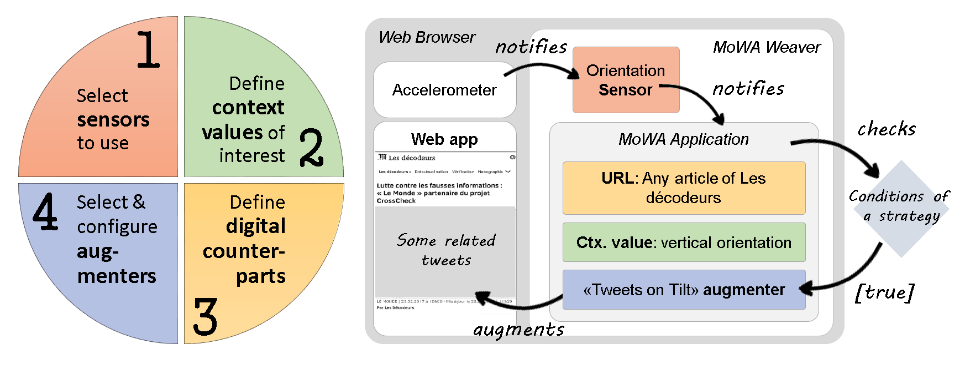
\includegraphics[width=\textwidth]{fig1.png}
\caption{Main stages of the authoring process and the expected application execution} \label{fig1}
\end{figure}

\section{A motivational scenario}
Wayra is a regular reader of \textit{Les Decodeurs}, a section of \textit{Le Monde} specialised in fact-checking and contextualization of popular assertions. She reads it daily on her phone, and sometimes she wants to know what people say about a concrete topic. In Figure~\ref{fig1}, Wayra is reading about “CrossCheck”(a), but the article has just two comments at the bottom of the page (b). She wants to read more opinions so, in this kind of situation, she used to copy the title, open a new tab, visit Twitter and perform a search using the copied text as keywords. However, this process became tedious for her and she eventually stopped doing it. She would like to retrieve tweets in the same context of the article easily. Besides, the extra interactions make her feel uncomfortable to perform it with a single hand, and she would like to use single-handed tilting gestures to show and hide an extra section with related tweets at the top of the article, as in steps “c” and “d”.

\begin{figure}
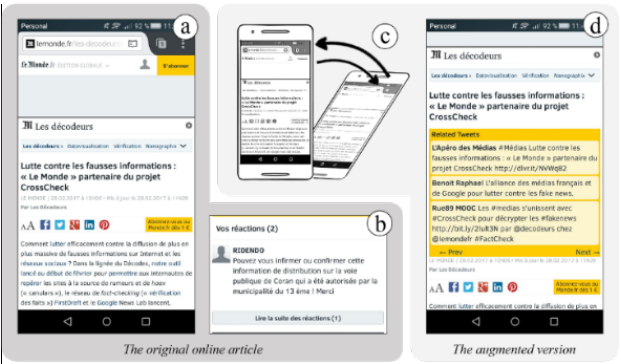
\includegraphics[width=\textwidth]{fig2.png}
\caption{The original mobile Web site and the augmented version} \label{fig2}
\end{figure}

MoWA authoring empowers Wayra to create her own solution; Figure 3 shows the screenshots of the main stages of the process. It starts when the user opens the tool in the browser (0) and the full-screen mode is enabled. He chooses to create a new application and sets up some base data. Then, he selects his required sensors (1), and manages the context values of interest according to the selected sensor, as an orientation in (2). In such a concrete case, values for the axes are automatically updated; the user should move the device to the desired position and save it. Then, he defines at least one digital counterpart in (3) and eventually sets up the augmentation layer (4).

\begin{figure}
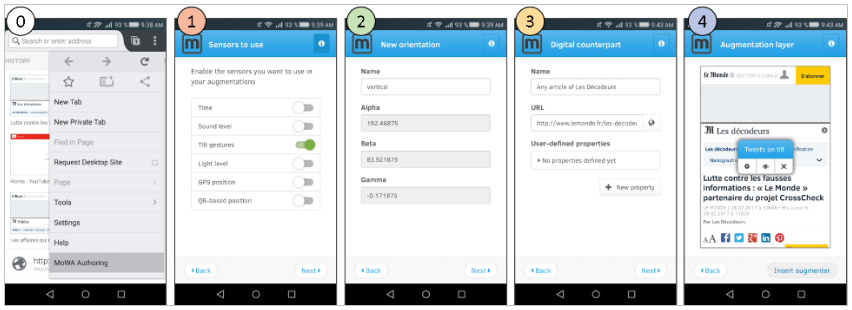
\includegraphics[width=\textwidth]{fig3.png}
\caption{Main stages of the authoring process through the tool} \label{fig3}
\end{figure}

He can use as many augmenters as required. The last screenshot shows that an instance of the \textit{TweetsOnTilt} augmenter has been created. This augmenter is capable of showing related Tweets through a sliding down effect that –as a physical metaphor of an object sliding on the surface– makes the interaction memorable for the user. The augmenter just requires the user to pick a DOM element for generating an XPath, so each time the document is loaded, the DOM element can be retrieved and its textContent attribute can be used as the keywords to search on Twitter. 

\section{Conclusions and Further Work}
This paper presents MoWA Authoring, a platform supporting an approach for enhancing Web applications with mobile features. The tool currently supports a set of extensible and specialised sensors, context types and augmenters for covering scenarios in different domains. We are currently extending the platform with new augmenters to provide the end users with a broader spectrum of specific behaviours and making them available from a repository for easy maintenance. For more information about the project, please visit the site of the project\footnote{footnotes working fine}.

\section{Acknowledgments}
This work was supported by the \guillemotleft STIC-AMSUD\guillemotright\thinspace Project named \guillemotleft WAMAW-OUR: Web Augmentation Methods for Adapting Web Sites for Supporting Opportunistic User Requirements\guillemotright.

\section{References}
% ---- Bibliography ----
%
% BibTeX users should specify bibliography style 'splncs04'.
% References will then be sorted and formatted in the correct style.
\bibliographystyle{unsrt}
\renewcommand{\refname}{}
\bibliography{ref}
\end{document}
